% PDF p. 131
\section{庞加莱引理和庞加莱映射的解释与意义}
\label{sec:3.8}
\subsection{引言}
庞加莱引理是微分几何和拓扑学的基本结果，在研究微分形式和德拉姆上同调（de Rham cohomology）时尤其重要。它断言在某些区域中，每个闭微分形式（closed differential form）都是恰当的（exact）。这一引理在数学和物理学中有深远影响，有助于理解电磁学中的势、微分方程理论等概念。

庞加莱映射（Poincaré map）又称首次回归映射（first return map），来自动力系统和微分方程。它把连续的流化为离散映射，因而可用于分析动力系统的定性行为。庞加莱映射和庞加莱引理都以法国数学家亨利·庞加莱（Henri Poincaré）命名，在各自领域均有重要作用。两个概念之间没有直接的数学联系。

\needspace{6\baselineskip}
\subsection{庞加莱引理}
\begin{statement}{定义 3.8}{$\R^n$ 中的星形（或可缩）开子集}
设 $U\subset\R^n$ 是一个区域。若对于每个 $x\in\R^n$，线段 $\overline{x_0x}$ 全部包含在 $U$ 内，就称 $U$ 关于 $x_0\in\R^n$ 是星形的（star-shaped）。%
\translatornote{原书将量词写为 $x\in\R^n$。星形性的条件应为对每个 $x\in U$。星形开集可以沿线段收缩到星心，因而可缩（contractible），反过来一般不成立。本定义的编号 3.8 与 3.5.2.1 节中的定义 3.8 重复，保留原号。}%
若 $U$ 关于某一点是星形的，就称 $U$ 为星形区域。图 \ref{fig:3.4} 显示了一个星形开子集，其中的阴影区域 $D$ 关于点 $x_0$ 是星形的，因为将 $x_0$ 与任一边界点相连的线段完全位于 $D$ 内。黑色曲线表示边界，黑色射线示意其中几条线段。%
\translatornote{图中边界为蓝色，线段为红色。对开集，线段除边界端点外可位于内部。}
\end{statement}
\begin{figure}[htbp]
\centering
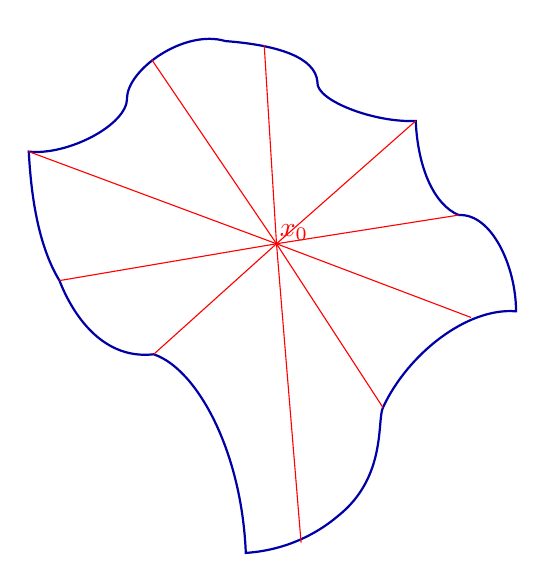
\begin{tikzpicture}[x=.026cm,y=-.026cm]
\coordinate (star) at (121,100);
\draw[blue!65!black,thick]
  (0,55) .. controls (19,57) and (48,42) .. (48,29)
  .. controls (48,15) and (76,-5) .. (96,1)
  .. controls (122,3) and (140,9) .. (141,21)
  .. controls (140,30) and (169,41) .. (189,40)
  .. controls (190,63) and (198,81) .. (210,86)
  .. controls (226,85) and (238,111) .. (238,133)
  .. controls (214,131) and (185,154) .. (173,180)
  .. controls (170,186) and (175,214) .. (151,233)
  .. controls (138,244) and (122,250) .. (106,251)
  .. controls (104,201) and (82,161) .. (61,154)
  .. controls (34,157) and (20,131) .. (15,118)
  .. controls (4,100) and (1,74) .. cycle;
\foreach \starend in {(0,55),(60,10),(115,3),(189,40),(210,86),
  (216,136),(173,180),(133,246),(61,154),(15,118)}
  \draw[red] (star)--\starend;
\node[red,above right,inner sep=1pt] at (star) {$x_0$};
\end{tikzpicture}

\FigureCaption{3.4}{一个星形开子集。}
\end{figure}

% PDF p. 132
\subsubsection{闭微分形式}
\begin{statement}{定义 3.9}{}
若微分形式 $\omega$ 的外微分为零，即 $d\omega=0$，则称 $\omega$ 是闭的。

闭形式在拓扑学和几何学中作用重要，在德拉姆上同调中尤其如此。它们也与物理学中的守恒量和势有关。下面给出不同维数和不同情形中的几个闭微分形式的例子。
\end{statement}

\begin{statement}{例 3.17}{}
\noindent\textbf{作为闭 0-形式的常函数}\par
0-形式就是流形 $M$ 上的光滑函数 $f$。由于函数的外微分就是它的微分，有 $df=0$ 当且仅当 $f$ 为常函数。%
\translatornote{在不连通的流形上，$df=0$ 只保证 $f$ 在每个连通分支上为常数。}
\end{statement}

\begin{statement}{例 3.18}{}
\noindent\textbf{函数的微分是闭 1-形式}\par
任意光滑函数 $f$ 的微分 $df$ 都是闭 1-形式，因为
\[
  d(df)=d^2f=0,
\]
即连续施行两次外微分 $d$ 总是得到零。

\noindent\textbf{示例 $f=f(x,y)$}
\[
  df=\frac{\partial f}{\partial x}\,dx+\frac{\partial f}{\partial y}\,dy.
\]
\noindent\textbf{计算外微分}
\begin{align*}
  d(df)&=d\!\left(\frac{\partial f}{\partial x}\right)\wedge dx
        +d\!\left(\frac{\partial f}{\partial y}\right)\wedge dy,\\
  &=\left(\frac{\partial^2 f}{\partial x^2}\,dx
          +\frac{\partial^2 f}{\partial x\partial y}\,dy\right)\wedge dx
     +\left(\frac{\partial^2 f}{\partial y\partial x}\,dx
          +\frac{\partial^2 f}{\partial y^2}\,dy\right)\wedge dy,\\
  &=\frac{\partial^2 f}{\partial x\partial y}\,dy\wedge dx
    +\frac{\partial^2 f}{\partial y\partial x}\,dx\wedge dy,\\
  &=\left(-\frac{\partial^2 f}{\partial x\partial y}
     +\frac{\partial^2 f}{\partial y\partial x}\right)\,dx\wedge dy=0.
\end{align*}
\end{statement}

\begin{statement}{例 3.19}{$\R^2$ 上的标准面积形式是闭 2-形式}
考虑 2-形式
\[
  \omega=dx\wedge dy.
\]
% PDF p. 133
\noindent\textbf{计算它的外微分}
\[
  d\omega=d(dx\wedge dy)=d(dx)\wedge dy-dx\wedge d(dy)=0-0=0,
\]
因为 $d(dx)=0$ 且 $d(dy)=0$。

\noindent\textbf{解释}
\begin{itemize}
\item $\omega$ 表示 $\R^2$ 中的标准面积元。
\item 它是闭的，在曲面积分中十分重要。
\end{itemize}
\end{statement}

\begin{statement}{例 3.20}{圆 $S^1$ 上的闭 1-形式}
在以角度 $\theta$ 参数化的圆 $S^1$ 上，令
\[
  \omega=d\theta.
\]
由于 $d(d\theta)=0$，$\omega$ 是闭 1-形式。

\noindent\textbf{说明}
\begin{itemize}
\item $\omega$ 在 $S^1$ 上并不恰当，因为不存在全局定义的函数 $f$ 使 $df=\omega$。
\item 这是由 $S^1$ 的非平凡拓扑所致。
\end{itemize}
\end{statement}

\begin{statement}{例 3.21}{形式 $\omega=\dfrac{-y}{x^2+y^2}\,dx+\dfrac{x}{x^2+y^2}\,dy$}
\noindent\textbf{定义在 $\R^2\setminus\{0,0\}$ 上}
\[
  \omega=\frac{-y}{x^2+y^2}\,dx+\frac{x}{x^2+y^2}\,dy.
\]
\noindent\textbf{计算 $d\omega$}\par
计算偏导数可得
\[
  d\omega=0.
\]
\noindent\textbf{解释}
\begin{itemize}
\item $\omega$ 在 $\R^2\setminus\{0,0\}$ 上是闭的，但不恰当。
\item 它对应于极坐标中的角形式 $d\theta$。
\end{itemize}
\end{statement}

\begin{statement}{例 3.22}{$\R^3\setminus\{0,0,0\}$ 上的闭 2-形式}
考虑 2-形式
\[
  \omega=\frac{x\,dy\wedge dz+y\,dz\wedge dx+z\,dx\wedge dy}
                 {(x^2+y^2+z^2)^{3/2}}.
\]
\noindent\textbf{计算 $d\omega$}\par
首先定义
\begin{gather*}
 F_1(x,y,z)=\frac{x}{(x^2+y^2+z^2)^{3/2}},\qquad
 F_2(x,y,z)=\frac{y}{(x^2+y^2+z^2)^{3/2}},\\
 F_3(x,y,z)=\frac{z}{(x^2+y^2+z^2)^{3/2}}.
\end{gather*}
% PDF p. 134
\noindent\textbf{计算}
\begin{gather*}
 \frac{\partial F_1}{\partial x}
 =\frac{x^2+y^2+z^2-3x^2}{(x^2+y^2+z^2)^{5/2}},\quad
 \frac{\partial F_2}{\partial y}
 =\frac{x^2+y^2+z^2-3y^2}{(x^2+y^2+z^2)^{5/2}},\\
 \frac{\partial F_3}{\partial z}
 =\frac{x^2+y^2+z^2-3z^2}{(x^2+y^2+z^2)^{5/2}},
\end{gather*}
\begin{align*}
 d\omega
   &=\frac{\partial F_1}{\partial x}\,dx\wedge dy\wedge dz
    +\frac{\partial F_2}{\partial y}\,dy\wedge dz\wedge dx
    +\frac{\partial F_3}{\partial z}\,dz\wedge dx\wedge dy,\\
   &=\frac{\partial F_1}{\partial x}\,dx\wedge dy\wedge dz
    +\frac{\partial F_2}{\partial y}\,dx\wedge dy\wedge dz
    +\frac{\partial F_3}{\partial z}\,dx\wedge dy\wedge dz,\\
   &=\frac{3(x^2+y^2+z^2)-3(x^2+y^2+z^2)}
           {(x^2+y^2+z^2)^{5/2}}\,dx\wedge dy\wedge dz=0.
\end{align*}
\noindent\textbf{解释}
\begin{itemize}
\item 这一形式与球面坐标中的立体角有关。
\item 由于 $\R^3\setminus\{0,0,0\}$ 的拓扑，它是闭的，但不恰当。
\end{itemize}
\end{statement}

\begin{statement}{例 3.23}{流形上的体积形式}
设 $M$ 为 $n$ 维有向流形，具有体积形式 $\omega$
\begin{equation*}
  \omega=\sqrt{\det(g_{ij})}\,dx^1\wedge dx^2\wedge\cdots\wedge dx^n.
  \tag{3.3}\label{eq:3.3}
\end{equation*}
其中 $g_{ij}$ 是度量张量。

\noindent\textbf{若流形平坦且度量为常量，}
\[
  d\omega=0,
\]
所以 $\omega$ 是一个闭 $n$-形式。
\end{statement}

\begin{statement}{例 3.24}{环面 $T^2$ 上的闭形式}
在以角度 $(\theta,\varnothing)$ 参数化的环面上，$\theta$ 是环绕 $xy$ 平面的角，$\varnothing$ 是 $xy$ 平面内绕 $z$ 轴的角。环面可参数化为
\begin{align*}
  x&=R\cos\varnothing+r\cos\theta\cos\varnothing,\\
  y&=R\sin\varnothing+r\cos\theta\sin\varnothing,\\
  z&=r\sin\theta.
\end{align*}
\begin{enumerate}
\item \textbf{1-形式。}
\[
  \omega_1=d\theta,\qquad \omega_2=d\varnothing.
\]
两者均为闭形式，因为 $d(d\theta)=d(d\varnothing)=0$。
% PDF p. 135
\item \textbf{2-形式。}
\[
  \omega=d\theta\wedge d\varnothing.
\]
计算 $d\omega$
\[
  d\omega=d(d\theta\wedge d\varnothing)=0.
\]
\end{enumerate}

\noindent\textbf{说明}
\begin{itemize}
\item 这些形式反映了环面的周期性结构。
\item 由于环面的拓扑，这两个 1-形式并不恰当。
\end{itemize}
\end{statement}

\subsubsection{恰当微分形式}
\begin{statement}{定义 3.10}{恰当微分形式}
若存在微分形式 $\eta$ 使 $\omega=d\eta$，则称微分形式 $\omega$ 是恰当的。

恰当微分形式（exact differential form）是可以写成另一个微分形式的外微分的微分形式。也就是说，当且仅当存在微分形式 $\eta$ 使得
\[
  \omega=d\eta
\]
时，微分形式 $\omega$ 是恰当的。

恰当形式总是闭的，即 $d\omega=0$，因为连续施行两次外微分得到零（$d^2=0$）。逆命题则不一定成立，某些闭形式并不恰当。每个闭形式是否都恰当取决于流形的拓扑，这是德拉姆上同调研究的问题。

下面给出不同维数和不同情形中的几个恰当微分形式的例子。
\end{statement}

\begin{statement}{例 3.25}{作为恰当 1-形式的函数微分}
令 $f(x,y)=x^2y$ 定义在 $\R^2$ 上。$f$ 的微分为
\[
  \omega=df=2xy\,dx+x^2\,dy.
\]
这里的 $\omega$ 是恰当 1-形式，因为它是 $f$ 的外微分。
\end{statement}

\begin{statement}{例 3.26}{涉及三角函数的恰当 1-形式}
考虑 $f(x,y)=\tan^{-1}\!\left(\dfrac{y}{x}\right)$。为避免不连续，把它定义在去掉 $x$ 轴负半轴的 $\R^2$ 上。%
\translatornote{在这一带割线的区域上应选取连续的极角分支，原式的 $\tan^{-1}(y/x)$ 须按象限延拓，且区域不含原点。}

\noindent\textbf{计算微分}
\[
  \omega=df=-\frac{y}{x^2+y^2}\,dx+\frac{x}{x^2+y^2}\,dy.
\]
所以 $\omega$ 是恰当 1-形式。
\end{statement}

% PDF p. 136
\begin{statement}{例 3.27}{由 $\R^3$ 中的 1-形式得到恰当 2-形式}
令 $\eta=x\,dy+y\,dz+z\,dx$ 为 $\R^3$ 上的 1-形式。计算其外微分
\[
  \omega=d\eta=dx\wedge dy+dy\wedge dz+dz\wedge dx.
\]
$\omega$ 是恰当 2-形式，因为 $\omega=d\eta$。
\end{statement}

\begin{statement}{例 3.28}{$\R^n$ 上的恰当 1-形式}
令 $f(x)=x_1x_2\cdots x_n$ 定义在 $\R^n$ 上。其微分为
\[
  \omega=df=\sum_{i=1}^n\left(\prod_{j\ne i}x_j\right)dx_i.
\]
$\omega$ 是一个恰当 1-形式。
\end{statement}

\begin{statement}{例 3.29}{$\R^2$ 上的恰当 2-形式}
令 $\eta=x^3\,dy$ 为 $\R^2$ 上的 1-形式。则
\[
  \omega=d\eta=3x^2\,dx\wedge dy.
\]
所以 $3x^2\,dx\wedge dy$ 是恰当 2-形式。
\end{statement}

\begin{statement}{例 3.30}{电磁学中的恰当形式}
在静电学中，电场 $E$ 是保守的，可以用电势 $V$ 的梯度表示
\begin{equation*}
  E=-\nabla V.
  \tag{3.4}\label{eq:3.4}
\end{equation*}
\noindent\textbf{对应的 1-形式为}
\[
  \omega=-dV.
\]
由于 $\omega=d(-V)$，它是一个恰当 1-形式。
\end{statement}

\begin{statement}{例 3.31}{恰当 2-形式}
令 $\eta=(xy)\,dz$ 为 $\R^3$ 上的 1-形式。则
\[
  \omega=(y\,dx+x\,dy)\wedge dz=y\,dx\wedge dz+x\,dy\wedge dz.
\]
所以 $\omega$ 是恰当 2-形式，因为 $\omega=d\eta$。
\end{statement}

\begin{statement}{例 3.32}{$\R^n$ 上的恰当体积形式}
在 $\R^n$ 中，考虑函数 $f(x)=\dfrac1n x_1x_2\cdots x_n$。它的微分 $df$ 为
\[
  df=\sum_{i=1}^n\left(\frac1n\prod_{j\ne i}x_j\right)dx_i.
\]
% PDF p. 137
考虑以下 $n$-形式
\begin{equation*}
  \omega=d\bigl(f\,dx^1\wedge dx^2\wedge\cdots\wedge dx^{n-1}\bigr).
  \tag{3.5}\label{eq:3.5}
\end{equation*}
这个 $\omega$ 是一个恰当 $n$-形式。
\end{statement}

\begin{statement}{例 3.33}{圆 $S^1$ 上的恰当形式}
在 $S^1$ 上考虑全局定义的函数 $f(\theta)=\sin\theta$，其中 $\theta$ 是参数化 $S^1$ 的角。则
\[
  \omega=df=\cos\theta\,d\theta.
\]
此处的 $\omega$ 是 $S^1$ 上的恰当 1-形式。
\end{statement}

\subsection{庞加莱引理}
\subsubsection{引理的陈述}
设 $U$ 是 $\R^n$ 的星形（或可缩）开子集，并且原点 $0\in U$。对于 $U$ 上定义的任意微分形式 $\omega$，%
\translatornote{引理适用于正次数微分形式。以下沿 $x\mapsto tx$ 的证明要求 $U$ 关于原点星形，即每条从原点到 $x\in U$ 的线段都在 $U$ 内。}
\begin{itemize}
\item 如果 $\omega$ 是闭的，即 $d\omega=0$，
\item 那么 $\omega$ 是恰当的，即存在微分形式 $\eta$ 使 $\omega=d\eta$。
\end{itemize}
用符号表示，在 $U$ 上有
\begin{equation*}
  d\omega=0\ \Longrightarrow\ \omega=d\eta.
  \tag{3.6}\label{eq:3.6}
\end{equation*}

\noindent\textbf{直观解释}\par
庞加莱引理告诉我们，在“简单”的区域中（例如没有孔洞的星形区域），所有闭形式都是恰当的。这意味着，如果某个微分形式局部看起来没有“扭转”或“旋转”（即 $d\omega=0$），实际上就能在全局把它表示成另一个形式的外微分。

\begin{statement}{例 3.34}{}
考虑函数 $f\colon\R^n\to\R$，其中 $f(x)=\lVert x\rVert^2=x_1^2+x_2^2+\cdots+x_n^2$。于是
\begin{itemize}
\item 微分 $df=2x_1\,dx_1+2x_2\,dx_2+\cdots+2x_n\,dx_n$。
\item 1-形式 $\omega=df$ 是恰当的，因为它是 $f$ 的外微分。
\item 由于 $d\omega=d(df)=0$（因为 $d^2=0$），$\omega$ 也是闭的。
\end{itemize}
在这种情形中，庞加莱引理确认了 $\omega$ 是闭的便意味着它是恰当的。
\end{statement}

% PDF p. 138
\subsubsection{庞加莱引理的证明概要}
\paragraph{证明思路}
证明的做法是显式构造一个形式 $\eta$，使得 $\omega=d\eta$。在星形区域内，沿从固定点 $x_0=0$ 到动点 $x$ 的直线对 $\omega$ 积分。

对每个 $k\geq 1$，定义线性算子
\[
  (H\omega)(x)=\int_0^1 t^{k-1}(i_X\omega)(tx)\,dt,
\]
其中
\[
  X_x=\sum_{i=1}^n X^i\frac{\partial}{\partial x^i}\qquad
  \text{（点 $x$ 处的径向向量场）。}
\]
$i_X\omega$ 是内积（interior product）。把 $X$ 代入形式 $\omega$ 的第一个变量，其次数便从 $k$ 降为 $k-1$（见附录 3A）。%
\translatornote{要使同伦恒等式成立，积分中的缩并应取在 $tx$ 处的 $\omega$ 与固定向量 $x$，即 $i_{X_x}\omega_{tx}$，其中用欧氏坐标识别各点切空间。若把 $i_X\omega$ 作为与径向场的逐点缩并，则 $X_{tx}=tX_x$，对 $t>0$ 应将权重改为 $t^{k-2}$。}

由于 $t\in[0,1]$ 时每个点 $tx$ 都在 $U$ 内（由星形假设），积分有定义，而且 $H\omega$ 是 $U$ 上的光滑 $(k-1)$-形式。

\paragraph{同伦公式}
对于次数 $k\geq1$ 的每个微分 $k$-形式 $\omega$，
\begin{equation*}
  d(H\omega)+H(d\omega)=\omega.
  \tag{3.7}\label{eq:3.7}
\end{equation*}
特别地，如果 $\omega$ 是闭的（$d\omega=0$），那么
\[
  \omega=d(H\omega),
\]
所以 $\omega$ 是恰当的，其原形式（primitive）为 $\eta\coloneqq H\omega$。下面证明同伦公式。

\paragraph{同伦公式的证明}
证明同伦公式之前，先引入拉回的概念。

\begin{statement}{定义 3.11}{拉回}
\noindent\textbf{给定}
\begin{itemize}
\item 光滑流形 $M$。
\item 光滑映射 $\Phi_t\colon M\to M$，例如 $M$ 上向量场 $V$ 生成的流。
\item $M$ 上次数为 $k$ 的微分形式 $\omega$。
\end{itemize}
流 $\Phi_t$ 对微分形式 $\omega$ 的拉回如下。
\begin{itemize}
\item \textbf{起点 $x_0$。} 假定 $x_0$ 是流形 $M$ 上的初始点。
\item \textbf{流的路径 $\Phi_t(x_0)$。} 随时间 $t$ 变化得到的一系列点构成流 $\Phi_t(x_0)$ 描出的路径，路径的方向由向量场 $V$ 决定。
% PDF p. 139
\item \textbf{微分形式 $\omega$。} 假定在终点 $\Phi_t(x_0)$ 处对 $\omega$ 求值。
\item \textbf{拉回 $\Phi_t^*\omega$。} 把形式 $\omega$ 拉回到初始点 $x_0$，相当于把 $\omega$ 从 $\Phi_t(x_0)$ 移回到 $x_0$。
\begin{enumerate}
\item \textbf{沿直线同伦拉回。}

先说明同伦（homotopy）。同伦是映射空间 $\operatorname{Map}(X,Y)$ 中从第一个函数到第二个函数的一条路径。

定义 $F\colon[0,1]\times U\to U$，$F(t,x)=tx$。

记投影 $\pi\colon[0,1]\times U\to U$，并记 $i_t\colon U\to[0,1]\times U$，$x\mapsto(t,x)$。

注意 $F\circ i_t=t\operatorname{id}_U$，其中 $\operatorname{id}_U$ 是集合（或流形）$U$ 上的恒等映射，即
\[
  \operatorname{id}_U\colon U\to U,\qquad
  \operatorname{id}_U(x)=x\quad\text{对每个 $x\in U$。}
\]
因而它保持每个点不变。它的微分是各切空间上的恒等映射，雅可比矩阵是单位矩阵，并且是限制在 $U$ 上的映射复合的单位元。
\item \textbf{嘉当公式（Cartan's magic formula）。}%
\translatornote{原书此处及以下数处拼作 Cartin。本节式 \eqref{eq:3.8} 是嘉当公式。}

先引入几个理解该定理所需的记号。
\end{enumerate}
\item \textbf{包含映射（inclusion map）。}

对于固定参数 $t$（通常 $t\in[0,1]$），定义
\[
  i_t\colon U\to[0,1]\times U,\qquad i_t(x)=(t,x).
\]
它把 $U$ 嵌入为切片 $\{t\}\times U$。
\item \textbf{用映射 $F$ 拉回形式 $\omega$。}

给定光滑映射 $F\colon[0,1]\times U\to U$ 和 $U$ 上的微分形式 $\omega$，在 $[0,1]\times U$ 上定义拉回形式 $F^*\omega$
\[
  (F^*\omega)_{(t,x)}(v_1,\dots,v_k)
    =\omega_{F(t,x)}\bigl(dF_{(t,x)}v_1,\dots,dF_{(t,x)}v_k\bigr).
\]
\end{itemize}
\end{statement}

\begin{statement}{例 3.36}{}
设 $t\in(0,1)$，$U\subset\R^2$ 为单位正方形。定义映射
\[
  F\colon[0,1]\times U\to U,\qquad F(t,x,y)=(tx,ty).
\]
在定义域上采用坐标 $(t,x,y)$，在 $\R^2$ 上采用标准坐标 $(X^1,X^2)=(X,Y)$。

\noindent\textbf{雅可比（微分）矩阵 $dF_{(t,x,y)}$}\par
将 $F$ 写成 $(F^1,F^2)$，其中
\[
  F^1(t,x,y)=tx,\qquad F^2(t,x,y)=ty.
\]
\noindent\textbf{求偏导数}
\begin{align*}
  \partial_tF^1&=x,&\partial_xF^1&=t,&\partial_yF^1&=0,\\
  \partial_tF^2&=y,&\partial_xF^2&=0,&\partial_yF^2&=t.
\end{align*}
% PDF p. 140
因此
\[
  dF_{(t,x,y)}
  =\begin{pmatrix}\partial_tF^1&\partial_xF^1&\partial_yF^1\\
                   \partial_tF^2&\partial_xF^2&\partial_yF^2\end{pmatrix}
  =\begin{pmatrix}x&t&0\\y&0&t\end{pmatrix}.
\]
这个线性映射作用在切向量 $(\delta t,\delta x,\delta y)=T_{(t,x,y)}([0,1]\times U)$ 上。%
\translatornote{原书切向量与切空间之间用等号，应理解为切向量属于该切空间。}

\noindent\textbf{将 $dF_{t,x,y}$ 作用于具体的向量 $v_1$}\par
设 $v_1=(\delta_t,\delta_x,\delta_y)=(0,a,0)$，该微分在 $v_1$ 上的作用为
\[
  dF_{(t,x,y)}(v_1)
  =\begin{pmatrix}x&t&0\\y&0&t\end{pmatrix}
   \begin{pmatrix}0\\a\\0\end{pmatrix}
  =\begin{pmatrix}ta\\0\end{pmatrix}\in T_{F(t,x,y)}\R^2.
\]
取 $t=0.6$ 和 $a=0.25$，得到
\[
  dF_{(0.6,x,y)}(v_1)=(0.15,0).
\]
从几何上看，$v_1$ 在 $U$ 中指向 $x$ 方向。在 $F$ 的作用下，所有水平方向的长度都按因子 $t$ 缩放，因而像向量缩短为原来的 $t$ 倍，仍指向水平方向。

\noindent\textbf{目标空间上的 2-形式}\par
选用通常的面积形式 $\omega=dx\wedge dy$。回忆 $[0,1]\times U$ 上的拉回形式 $F^*\omega$ 定义为
\[
  (F^*\omega)_{(t,x)}(v_1,\dots,v_k)
    =\omega_{F(t,x)}\bigl(dF_{(t,x)}v_1,\dots,dF_{(t,x)}v_k\bigr).
\]
在这个例子中，
\[
  (F^*\omega)_{(t,x,y)}(v_1,v_2)
    =\omega_{F(t,x,y)}\bigl(dF_{(t,x,y)}v_1,dF_{(t,x,y)}v_2\bigr),
\]
其中
\[
  v_1=(v_1^x,v_1^y),\qquad v_2=(v_2^x,v_2^y).
\]
\[
  dF_{(t,x,y)}v_1=(tv_1^x,tv_1^y),\qquad
  dF_{(t,x,y)}v_2=(tv_2^x,tv_2^y).
\]
因此
\begin{align*}
 &\omega_{F(t,x,y)}\bigl(dF_{(t,x,y)}v_1,dF_{(t,x,y)}v_2\bigr)\\
 &\qquad=\det\begin{pmatrix}dF_{(t,x,y)}v_1\\ dF_{(t,x,y)}v_2\end{pmatrix}
   =\det\begin{pmatrix}tv_1^x&tv_1^y\\tv_2^x&tv_2^y\end{pmatrix}\\
 &\qquad=t^2\det\begin{pmatrix}v_1^x&v_1^y\\v_2^x&v_2^y\end{pmatrix}.
\end{align*}
% PDF p. 141
按定义，拉回形式为%
\translatornote{这里的 $v_1,v_2$ 都取在 $t$ 固定的切片上，时间分量为零。对乘积空间中任意切向量，$F^*(dx\wedge dy)=d(tx)\wedge d(ty)$ 还含有 $dt$ 项。}%
\[
  (F^*\omega)_{(t,x,y)}(v_1,v_2)
   =t^2\det\begin{pmatrix}v_1^x&v_1^y\\v_2^x&v_2^y\end{pmatrix}.
\]

\begin{itemize}
\item \textbf{微分形式的拉回。}

给定 $[0,1]\times U$ 上的形式 $\beta$，拉回 $i_t^*\beta$ 是将 $\beta$ 限制到该切片得到的 $U$ 上的形式
\begin{align*}
  (i_t^*\beta)_x(v_1,\dots,v_k)
    &=\beta_{(t,x)}\bigl(di_t(v_1),\dots,di_t(v_k)\bigr)\\
    &=\beta_{(t,x)}\bigl((0,v_1),\dots,(0,v_k)\bigr),
\end{align*}
其中
\[
  i_t\colon U\to[0,1]\times U,\qquad i_t(x)=(t,x).
\]
雅可比（微分）矩阵为
\[
  di_t(x)=\begin{pmatrix}0\\1\end{pmatrix}.
\]
因此
\[
  di_t(v_i)=\begin{pmatrix}0\\v_i\end{pmatrix},\qquad i=1,\dots,k,
\]
并且
\[
  (i_t^*\beta)_x(v_1,\dots,v_k)=\beta_{(t,x)}\bigl((0,v_1),\dots,(0,v_k)\bigr).
\]

\item \textbf{嘉当公式。}

对于 $U$ 上的微分形式 $\omega$，%
\translatornote{中间项应为 $i_t^*(\mathcal L_{\partial_t}F^*\omega)$，最右端的两项均应由 $i_t^*$ 拉回。3.8.3.2.3 节下文再次写出的公式及附录 3B 给出完整表达式。}%
\[
 \frac{d}{dt}(i_t^*F^*\omega)
   =i_t^*(\mathcal L_{\partial_t})
   =i_t^*\bigl(d(i_{\partial_t}F^*\omega)\bigr)+i_{\partial_t}dF^*\omega.
\]
嘉当公式常写成以下直观形式。对于每个向量场 $Z$ 和每个微分形式 $\omega$，
\begin{equation*}
  \mathcal L_Z\omega=d(i_Z\omega)+i_Z(d\omega).
  \tag{3.8}\label{eq:3.8}
\end{equation*}
因此，计算 $\mathcal L_Z\omega$ 的步骤如下。
\begin{enumerate}
\item 用 $Z$ 缩并 $\omega$（次数降 1），再求外微分。
\item 对 $\omega$ 求外微分（次数升 1），再作缩并。
\item 将两项相加。
\end{enumerate}
\item \textbf{$\R^2$ 中的具体例子。}

取坐标 $(x,y)$ 和向量场
\[
  Z=y\partial_x-x\partial_y.
\]
% PDF p. 142
取 1-形式
\[
  \alpha=x\,dy.
\]

\noindent\textbf{目标是计算 $\mathcal L_Z\alpha$。}

\begin{itemize}
\item 步骤 1。计算 $i_Z\alpha$。
\[
  \alpha(\partial_x)=0,\qquad \alpha(\partial_y)=x.
\]
于是
\begin{align*}
  i_Z\alpha&=\alpha(z)=\alpha(y\partial_x-x\partial_y)\\
  &=y\alpha(\partial_x)-x\alpha(\partial_y)=0-x\cdot x=-x^2.
\end{align*}

步骤 2。求缩并结果的外微分。
\[
  d(i_Z\alpha)=-2x\,dx.
\]

步骤 3。求 $\alpha$ 的外微分。
\[
  d\alpha=d(x\,dy)=dx\wedge dy.
\]

步骤 4。用 $Z$ 缩并 $d\alpha$。
\[
  i_Z(dx\wedge dy)=(dx\wedge dy)(y\partial_x-x\partial_y)=y\,dy+x\,dx.
\]

步骤 5。将两部分相加。
\[
  \mathcal L_Z\alpha=-2x\,dx+y\,dy+x\,dx=-x\,dx+y\,dy.
\]
\end{itemize}
\end{itemize}
下面用莱布尼茨法则（乘积法则）计算李导数 $\mathcal L_Z\alpha$
\begin{align*}
  \mathcal L_Z\alpha
   &=\mathcal L_Z(x\,dy)=(\mathcal L_Z x)\,dy+x\mathcal L_Z(dy)\\
   &=Z(x)\,dy+x\,d(\mathcal L_Z y)=Z(x)\,dy+x\,d(Z(y))\\
   &=(y\partial_x-x\partial_y)(x)\,dy+x\,d\bigl((y\partial_x-x\partial_y)(y)\bigr)\\
   &=y\,dy-x\,dx.
\end{align*}
这与上面的等式给出同一结果。第 4 章将正式证明嘉当公式。

下面用嘉当公式证明同伦公式。先回顾同伦算子（homotopy operator）$H$ 的定义。对 $U$ 上的 $k$-形式 $\omega$（$k\geq1$），令
\[
  (H\omega)(x)=\int_0^1 t^{k-1}(i_X\omega)(tx)\,dt,
\]
其中
\[
  X_x=\sum_{i=1}^n x^i\frac{\partial}{\partial x^i}
   \qquad\text{（点 $x$ 处的径向向量场）。}
\]
% PDF p. 143
\begin{itemize}
\item $i_X\omega$ 是内积。把 $X$ 代入形式 $\omega$ 的第一个变量，次数就从 $k$ 降至 $k-1$。
\item 由于 $t\in[0,1]$ 时 $tx$ 都在 $U$ 内（星形假设），积分有定义，且 $H\omega$ 是 $U$ 上的光滑 $(k-1)$-形式。
\end{itemize}

\noindent\textbf{同伦公式}\par
对于次数 $k\geq1$ 的每个微分 $k$-形式 $\omega$，下式成立
\[
  d(H\omega)+H(d\omega)=\omega.
\]
这一恒等式说明组合算子 $dH+Hd$ 在所有正次数形式上都是恒等算子。特别地，若 $\omega$ 是闭的（$d\omega=0$），则
\[
  \omega=d(H\omega),
\]
所以 $\omega$ 是恰当的，其原形式为 $\eta\coloneqq H\omega$。

\needspace{5\baselineskip}
\noindent\textbf{3. 同伦公式的证明}\par
\noindent\textbf{3.1 沿直线同伦拉回}\par
定义
\[
  F\colon[0,1]\times U\to U,\qquad F(t,x)=tx.
\]
记投影 $\pi\colon[0,1]\times U\to U$，以及 $i_t\colon U\to[0,1]\times U$，$x\mapsto(t,x)$。可以看到 $F\circ i_t=t\operatorname{id}_U$。

\noindent\textbf{3.2 嘉当公式}\par
对于 $U$ 上的微分形式 $\omega$，有（见附录 3B）
\[
  \frac{d}{dt}(i_t^*F^*\omega)=i_t^*(\mathcal L_{\partial_t}F^*\omega)
  =i_t^*\bigl(d(i_{\partial_t}F^*\omega)+i_{\partial_t}(dF^*\omega)\bigr).
\]

\noindent\textbf{3.3 将 $\partial_tF$ 与径向场联系起来}\par
将 $\partial_tF$ 与径向场等同%
\translatornote{原书此式前一等号有误。直接微分得 $\partial_tF(t,x)=x$。按欧氏坐标识别切空间后，这个向量是 $X_x$，等于 $t^{-1}X_{tx}$（$t>0$）。}%
\[
  \partial_tF(t,x)=X_{tx}=tX_x.
\]
注意
\[
  \int_0^1\frac{d}{dt}(i_t^*F^*\omega)\,dt
    =\left.i_t^*F^*\omega\right|_{t=1}-\left.i_t^*F^*\omega\right|_{t=0}
    =\omega-i_{t_0}^*F^*\omega.
\]
但 $i_{t_0}^*F^*\omega\equiv0$，因为 $F(0,x)=0$，任意正次数形式拉回到单点时都为零。
% PDF p. 144
因此
\begin{align*}
  \omega&=\int_0^1\frac{d}{dt}(i_t^*F^*\omega)\,dt,\\
   &=\int_0^1\Bigl[i_t^*\bigl(d(i_{\partial_t}F^*\omega)+i_{\partial_t}(dF^*\omega)\bigr)\Bigr]dt.
\end{align*}
把因子 $t^{k-1}$ 提出。当 $\omega$ 为 $k$-形式时，$i_{tX}\omega=t\,i_X\omega$，故上式可改写为（见附录 3B）%
\translatornote{若缩并向量按前注固定为 $x$，第二项的权重应为 $t^k$，因为 $d\omega$ 的次数是 $k+1$。附录 3B 将该项写作 $Hd\omega$。}%
\[
  \omega=d\left(\int_0^1 t^{k-1}i_X\omega(tx)\,dt\right)
     +\int_0^1 t^{k-1}i_X(d\omega)(tx)\,dt=dH\omega+Hd\omega.
\]
由此证明了同伦公式。
\end{statement}
